% For copyright and license information, see uiucthesis2021.dtx and derivatives.
\documentclass{uiucthesis2021}
\usepackage[utf8]{inputenc}
\usepackage[english]{babel}
\usepackage{csquotes}
\usepackage{microtype}
\usepackage{amsmath,amsthm,amssymb}
\usepackage[bookmarksdepth=3,linktoc=all,colorlinks=true,urlcolor=blue,
	linkcolor=blue,citecolor=blue]{hyperref}
\usepackage[capitalize]{cleveref}
\usepackage[style=phys,%
biblabel=brackets,%
chaptertitle=false,pageranges=false,%
maxnames=4,sorting=none]{biblatex}
%\usepackage[style=ieee]{biblatex}
\usepackage{physics}
\usepackage{subcaption}
\usepackage{tikz}
\usepackage{listings}
\usepackage{siunitx}
\usepackage{mhchem}
% \usepackage{ruledchapters}  % example of compliant heading format, uncomment to use

\usepackage{lipsum}  % just for placeholder code
\usepackage{pdfcomment}
\pdfcommentsetup{draft} %set to 'final' to prevent all comments from showing up

\usepackage{lineno}
\linenumbers

% uncomment the below to show a grid on all pages
% \usepackage[grid, gridunit=in, gridcolor=blue!40, subgridcolor=blue!20]{eso-pic}

\addbibresource{references.bib}
\begin{document}

\title{Probing parton distributions in proton with charmonium production with
	120 GeV proton beam at Fermilab}
\author{Ching Him Leung}
\department{Physics}
%\concentration{Coffee Studies}
\phdthesis
\degreeyear{2023}
\committee{
	Associate Professor Anne M Sickles , Chair\\
	Professor Jen-Chieh Peng, Director of Research\\
	Professor \\
	Professor }
\maketitle

\frontmatter

\begin{abstract}
E906/SeaQuest is a fixed-target experiment at Fermilab with a \SI{120}{\GeV} 
proton beam. Muon pairs with mass between \num{2} to \SI{9}{\GeV} from the 
interaction of proton beam with various targets has been detected. The primary 
goal of the experiment is to study the partonic structure of the nucleon. In 
particular, the charmonium production data can be used to probe both the quark 
content as well as the gluon content. The preliminary result from the analysis 
of the SeaQuest charmonium production data will be presented.  E1039/SpinQuest 
is a follow up experiment of SeaQuest. By utilizing a transversely polarized 
target,we could extend this study to the transverse momentum distribution of 
the partons. 
\pdfcomment{copied from prelim, needed to be rewritten}
\end{abstract}

\begin{dedication}
To Father and Mother.
\end{dedication}

\begin{acknowledgments}
This research is supported by National Science Foundation via grant No.XXXXXXX.

First and foremost I would like to thank my advisor, Prof. Jen-Chieh Peng, for 
his continuous support and assistance. I would also like to express my 
appreciation for his efforts and encouragement particularly during the 
challenge brought by the pandemic. 

I would also like to thank former graduate students Jason Dove and Shivangi 
Prasad for all their help. 

Finally, I would like to thank both the SeaQuest and SpinQuest collaborations. 
I would like to thank the SeaQuest collabration for all their work. I would 
also like to thank Kiu Liu of Los Almos National Lab and Rick Tesarak of 
for their help and guidance during my short stay in Fermilab.

\end{acknowledgments}



{
	\hypersetup{linkcolor=black}  % disable link coloring locally
	\tableofcontents
	% the Graduate College doesn't recommend including lot or lof
	%\listoftables
	\listoffigures
}


\mainmatter

\chapter{Introduction}
%\section{Theory}
\section {Internal structure of Nucleon}
\pdfcomment{magnetic moment of proton and neutron}
The first evident of nucleons being a composite particles comes form the 
measurement of their magnetic moment. For spin 1/2 elementary particles, the 
magnetic moment can be expressed as 
\begin{equation}
\mu = \frac{g}{i2}\mu_B ~~~~ \mu_B = \frac{e\hbar}{2m},
\end{equation}
with $g$ expected to be $2$. Such measurement was first carried out by Otto 
Stern in 1933. And they found that the $g$ factor for proton is significantly 
greater than $2$. Since the neutron is a neutral particle, it was expected that
to have a zero magnetic moment. Stern and his team would later found that the 
neutron moment to be non-zero, suggesting that proton and neutron are composite
particles.
\pdfcomment{find appropriate citation. The original paper on proton magnetic
	moment is in Germany which I can't read}

\pdfcomment{proton form factor can be determined from e-p elastic scattering,
	which is related to the charge distribution in proton and neutron}
In the 1950s, the proton form factor was measured using electron proton elastic
scattering experiments\cite{hofstadter1956}. The elastic scattering cross 
section can be expressed as 
\begin{equation}
\dv{\sigma}{\Omega} = \left(\dv{\sigma}{\Omega}\right)_{Mott}\left\{ 
	\frac{G_E^2\left(Q^2\right) + \frac{Q^2}{4M^2}G_M^2 \left(Q^2\right)}
	{1 + \frac{Q^2}{4M^2}} + \frac{Q^2}{2M^2} G^2_M{Q^2}\tan^2\frac{\theta}{2}
	\right\},
\end{equation}
where $G_E\left(Q^2\right)$ is known as the electric form factor and can be 
interpreted as the Fourier transform of the charged distribution. The deviation
of the neutron electric form factor from zero further demonstrating the 
composite nature of the nucleons.

\section {Deep Inelastic Scattering}
\label{sec:dis}
Evidence of the point-like constituents in the nucleon first came from the deep
inelastic scattering (DIS) experiments \cite{breidenbach1969}. 
\pdfcomment{colin-gross relation shows that the protons are made up of spin 1/2
	partons. This relation would be different if the spin of partons is 
	different}


\section{Parton Model}
\label{sec:parton}

\subsection{Gottfried Sum Rule}
\label{sec:gottfried}

\section{Drell-Yan Process}
\label{sec:DY}

\pdfcomment{factorization and universality of PDF, scaling plot for both DIS 
	and DY}

\subsection{E866/NuSea}
\label{sec:E866}

\section{Charmonium Production}
\label{sec:jpsi}
The mechanism for charmonium production can be separated into two parts, the 
production of heavy-quark pairs and the subsequent hadronization into 
quarkonium states. One of the early approaches is the Color Evaporation method 
(CEM)\cite{einhorn1975,bodwin1995,bodwin1997}. The heavy-quark pairs production
is expanded in terms of the strong coupling constant s and is calculated with 
perturbative QCD (pQCD). CEM then assumes a constant probability $F$ for the 
$c\bar{c}$ pairs to hadronize into different charmonium state and this 
probability is independent of the kinematics or the production subprocess. The 
charmonium production cross section in the CEM framework can be expressed as
\begin{equation}
\eval{\dv{\sigma}{x_{F}}}_{J/\psi\left(\psi^\prime\right)} =
	F_{J/\psi\left(\psi^\prime\right)} \sum_{i,j=q,\bar{q},g} \int_{2m_c}^{2m_D}
\end{equation}


\pdfcomment{CEM and NRCD}

\pdfcomment{what is physical significant of the nuclear dependence}



\chapter{SeaQuest Experiment}
\documentclass[../main.tex]{subfiles}
\begin{document}

\ifSubfilesClassLoaded{
	\mainmatter
	\setcounter{chapter}{1}
}{}

\chapter{SeaQuest Experiment}
\label{ch:seaquest}

\section{Introduction}
SeaQuest is a fixed-target experiment utilizing the \SI{120}{\GeV} proton beam
from the Fermilab Main Injector. Details of the SeaQuest spectrometer can be
found in Ref.\ \cite{aidala2019}. A schematics of the spectrometer is shown in
Fig.\ \ref{fig:spectrometer}. The target system consists of seven
interchangeable targets, including a flask with liquid hydrogen, a flask with
liquid deuterium,an empty flask (vacuum), solid carbon, iron, and tungsten
targets as well as a space with no target (air). The targets are interchanged
periodically to reduce systematic uncertainties in the measured cross section
ratios for different targets.

The spectrometer consists of two magnets and four tracking stations. FMag,
placed \SI{104}{\cm} downstream the target, is a \SI{5}{\m} solid iron magnet
that acts as the beam dump as well as a focusing magnet. It is then followed by
the first tracking stations. Stations 1, 2 and 3 each consists of plastic
scintillator hodoscopes and drift chambers. An open air dipole magnet (KMag) is
placed between station 1 and station 2. The vertical magnetic field from both
magnets bends the muons horizontally, allowing the measurement of the momentum
of the muons. Downstream of station 3, there is a 1 m iron wall acting as a
hadron absorber. Station 4 is located behind the hadron absorber and acts as a
muon identifier. Station 4 consists of a hodoscope array and 4 layers of
proportional tube planes. Tracks that pass through the hadron absorber and
produce hits on station 4 are assumed to be from muons.
\pdfmargincomment{Should there be a dedicated section on the spectrometer?}

\begin{figure}[htbp!]
	\centering
	\includegraphics[width=0.6\linewidth]{SeaQuestSpectrometer}
	\caption{schematics of the SeaQuest spectrometer. Taken from Ref.\
		\cite{aidala2019}}
	\label{fig:spectrometer}
\end{figure}


\section{Beam}
\pdfmargincomment{A brief description of the beam structure, how the beam intensity
	is monitor. And finally says that the varying instantaneous beam intensity
	allows us to do intensity extrapolation which will be discussed in next
	chapter}
The layout of the Fermilab accelerator complex is shown in Fig.\ \ref{fig:complex}.
SeaQuest received its \SI{120}{\GeV} proton beam from the Fermilab Main Injector.
The proton beam originate from a direct-extraction magnetron hydrogen ion source,
which produce a \SI{35}{\keV} negative hydrogen ion beam. It is then accelerated
to \SI{750}{\keV} using Radio-frequency Quadrupole. Then the Linac accelrate the
$H^-$ ions to \SI{400}{MeV}. The $H^-$ ions are then sent through a stripping foil
to remove the electrons. The resulting proton beam then circulates in the Booster
accelerator and accelerates to \SI{8}{\GeV}. The \SI{8}{\GeV} proton beam is
further accelerated by the Main Injector to \SI{120}{GeV}. The proton beam is
extracted from the Main Injector using a process known as resonant extraction to
provide a lower intensity beam over a 5 second spill. The extracted beam, which
is sent to SeaQuest, retains the the \SI{53.1}{\MHz} structure of the Main
Injector RF frequency, dividing hte beam in to ``RF buckets'' that are less than
\SI{2}{\ns} long and occur every \SI{18.8}{\ns}
\begin{figure}[htbp!]
	\centering
	\includegraphics[width=0.6\linewidth]{Fermilab-complex}
	\caption{Layout of the Fermilab accelerator complex. Taken from Ref.\ \cite{concept-book}}
	\label{fig:complex}
\end{figure}
However the number of protons in each bucket varies greatly during the spill, as
is shown in Fig.\ \ref{fig:intensity}.

The beam intensity is monitored using a Cerenkov counter, shown in Fig.\ \ref{fig:BIM}.
\begin{figure}[htbp!]
	\centering
	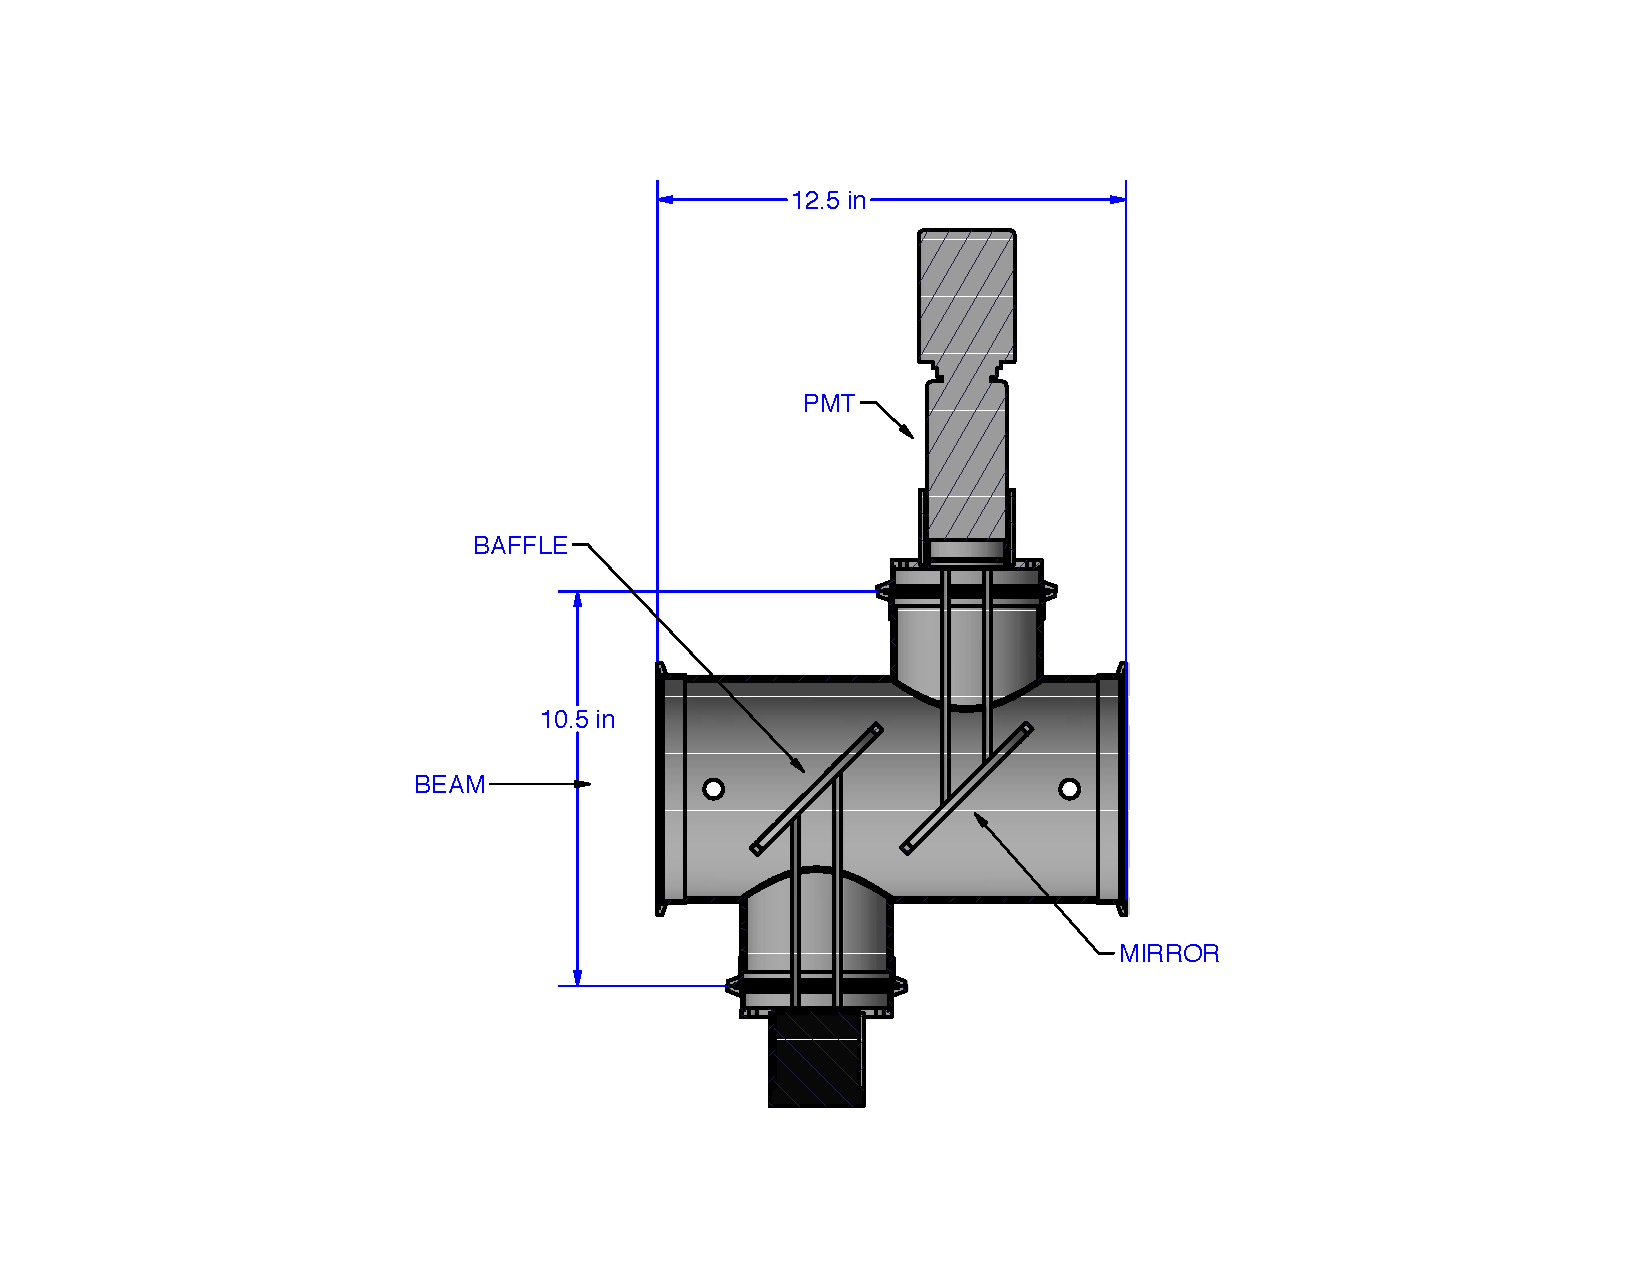
\includegraphics[width=0.6\linewidth]{BIMCerenkov}
	\caption{The Beam Intensity Monitor (BIM) Cerenkov counter. Taken from Ref.\
		\cite{aidala2019}.}
	\label{fig:BIM}
\end{figure}
This allows us the obtain the yield ratios as a function of the instantaneous
intensity, which will be discussed further in Sec.\ \ref{M-sec:extrapolation}


\begin{figure}[htpb!]
	\centering
	\includegraphics[width =0.8\linewidth, angle =270]{beam_intensity}
	\caption{The beam intensity measured by the Beam DAQ Cerenkov counter every
		bucket. Taken from Ref.\ \cite{aidala2019}}
	\label{fig:intensity}
\end{figure}

\section{Target}
\pdfmargincomment{list the properties of the targets. Some past thesis quoted the
	wrong number. Check PDG}

\ifSubfilesClassLoaded{ \printbibliography[heading=bibintoc,title={References}]}{}
\end{document}


\chapter{Analysis}
\section{Data Sets}

\section{Track Reconstruction}

\section{Event Selection}

\section{Intensity Extrapolation}

\section{Mass Spectrum Fitting}


\chapter{Results}
\documentclass[../main.tex]{subfiles}
\begin{document}

\ifSubfilesClassLoaded{
	\mainmatter
	\setcounter{chapter}{5}
}{}

\chapter{Results}
\label{ch:result}
\section{Drell-Yan Cross Section Ratio}
\subsection{Effect of the updated target contaimination correction}
As discussed in \cref{M-subsec:contamination}, an incorrect target contamination was used
in previous publication and the effect is shown in \cref{fig:contaimination_CSR}.
The overall effect is a roughtly \SI{2}{\percent} shift in the ratio.
\begin{figure}[h!]
	\centering
	\includegraphics[width=0.6\linewidth]{placeholder}
	\caption{The effect of the updated target contamination correction on the Drell-Y.an
		cross section. The overall effect is a roughly \SI{2}{\percent} shift in the ratio. }
	\label{fig:contaimination_CSR}
\end{figure}

\subsection{Comparison of massfit and extrapolation}
As shown in Ref.~\cite{dove2023} the Drell-Yan cross section extracted from the two methods
are consistent with each other.
\begin{figure}[h!]
	\centering
	\includegraphics[width=0.6\linewidth]{placeholder}
	\caption{Comparison of the extracted Drell-Yan cross section from the Run 2-3 data using the massfit
		and intensity extrapolation method.}
	\label{fig:CSR_Run2-3}
\end{figure}

\subsection{Results from Run 5-6 data}
\pdfmargincomment{run 5-6 compared with 2-3 and full data set}
\subsubsection{Potential cause of difference between massfit and intensity extrapolation}
It is possible the systematic uncertainties for the intensity extrapolation was
underestimated
\pdfcomment{chisq from multiple fit}

\subsection{Extraction of \texorpdfstring{$\bar{d}/\bar{u}$}{dbar/ubar}}
The $\sigma_{pd}/2\sigma_{pp}$ ratio is used by the NNPDF collaboration in
their PDF extraction\cite{ball2021} and their result is shown in Fig.\
\ref{fig:nnpdf_e906}.

\begin{figure}[htbp!]
	\centering
	\begin{subfigure}{0.45\linewidth}
		\includegraphics[width=\linewidth]{data_vs_theory_nnpdf40_e906}
		\caption{Calculated Drell-Yan cross section ratio.}
		\label{subfig:nnpdf_e906_csr}
	\end{subfigure}
	\begin{subfigure}{0.45\linewidth}
		\includegraphics[width=\linewidth]{placeholder}
		\caption{Extracted $\bar{d/}\bar{u}$ ratio.}
		\label{subfig:nnpdf_e906_x2}
	\end{subfigure}
	\caption{Comparison of NNPDF4.0\cite{ball2021} with the SeaQuest
		result\cite{dove2021}.}
	\label{fig:nnpdf_e906}
	\pdfmargincomment{Should be compared with the new result from run5-6 and full
		data set}
\end{figure}

\section{Charmonium Cross Section}
\pdfmargincomment{absolute cross section and cross section ratios; mean pT for
	jpsi as a function of root s}

\subsection{Massfit results}
The massfits in all $x_F$ bins are shown in \cref{fig:massfit_57-70_xF,fig:massfit_5-6_xF},
and the fits in the $P_T$ bins are shown in \cref{fig:massfit_57-70_pT,fig:massfit_5-6_pT}.
The two datasets are analyzed separately. The data in each bin is very well described by the fitting procedure
and the $J/\psi$ and $\psi'$ yields can be extracted from the massfits.
\begin{figure}[h]
	\centering
	\begin{subfigure}{0.4\linewidth}
		\includegraphics[width=0.9\linewidth]{massfit/run2-3/LH2/xF/LH2_xFbin0}
	\end{subfigure}
	\begin{subfigure}{0.4\linewidth}
		\includegraphics[width=0.9\linewidth]{massfit/run2-3/LD2/xF/LD2_xFbin0}
	\end{subfigure}\\
	\begin{subfigure}{0.4\linewidth}
		\includegraphics[width=0.9\linewidth]{massfit/run2-3/LH2/xF/LH2_xFbin1}
	\end{subfigure}
	\begin{subfigure}{0.4\linewidth}
		\includegraphics[width=0.9\linewidth]{massfit/run2-3/LD2/xF/LD2_xFbin1}
	\end{subfigure}\\
	\begin{subfigure}{0.4\linewidth}
		\includegraphics[width=0.9\linewidth]{massfit/run2-3/LH2/xF/LH2_xFbin2}
	\end{subfigure}
	\begin{subfigure}{0.4\linewidth}
		\includegraphics[width=0.9\linewidth]{massfit/run2-3/LD2/xF/LD2_xFbin2}
	\end{subfigure}\\
	\begin{subfigure}{0.4\linewidth}
		\includegraphics[width=0.9\linewidth]{massfit/run2-3/LH2/xF/LH2_xFbin3}
	\end{subfigure}
	\begin{subfigure}{0.4\linewidth}
		\includegraphics[width=0.9\linewidth]{massfit/run2-3/LD2/xF/LD2_xFbin3}
	\end{subfigure}\\
	\begin{subfigure}{0.4\linewidth}
		\includegraphics[width=0.9\linewidth]{massfit/run2-3/LH2/xF/LH2_xFbin4}
	\end{subfigure}
	\begin{subfigure}{0.4\linewidth}
		\includegraphics[width=0.9\linewidth]{massfit/run2-3/LD2/xF/LD2_xFbin4}
	\end{subfigure}
	\caption{Mass fit for run 2-3 data in each $x_F$ bin for both \ce{LH_2}(left) and \ce{LD_2}(right) targets. }
	\label{fig:massfit_57-70_xF}
\end{figure}

\begin{figure}[h]
	\centering
	\begin{subfigure}{0.4\linewidth}
		\includegraphics[width=0.9\linewidth]{massfit/run5-6/LH2/xF/LH2_xFbin0}
	\end{subfigure}
	\begin{subfigure}{0.4\linewidth}
		\includegraphics[width=0.9\linewidth]{massfit/run5-6/LD2/xF/LD2_xFbin0}
	\end{subfigure}\\
	\begin{subfigure}{0.4\linewidth}
		\includegraphics[width=0.9\linewidth]{massfit/run5-6/LH2/xF/LH2_xFbin1}
	\end{subfigure}
	\begin{subfigure}{0.4\linewidth}
		\includegraphics[width=0.9\linewidth]{massfit/run5-6/LD2/xF/LD2_xFbin1}
	\end{subfigure}\\
	\begin{subfigure}{0.4\linewidth}
		\includegraphics[width=0.9\linewidth]{massfit/run5-6/LH2/xF/LH2_xFbin2}
	\end{subfigure}
	\begin{subfigure}{0.4\linewidth}
		\includegraphics[width=0.9\linewidth]{massfit/run5-6/LD2/xF/LD2_xFbin2}
	\end{subfigure}\\
	\begin{subfigure}{0.4\linewidth}
		\includegraphics[width=0.9\linewidth]{massfit/run5-6/LH2/xF/LH2_xFbin3}
	\end{subfigure}
	\begin{subfigure}{0.4\linewidth}
		\includegraphics[width=0.9\linewidth]{massfit/run5-6/LD2/xF/LD2_xFbin3}
	\end{subfigure}\\
	\begin{subfigure}{0.4\linewidth}
		\includegraphics[width=0.9\linewidth]{massfit/run5-6/LH2/xF/LH2_xFbin4}
	\end{subfigure}
	\begin{subfigure}{0.4\linewidth}
		\includegraphics[width=0.9\linewidth]{massfit/run5-6/LD2/xF/LD2_xFbin4}
	\end{subfigure}
	\caption{Mass fit for run 5-6 data in each $x_F$ bin for both \ce{LH_2}(left) and \ce{LD_2}(right) targets. }
	\label{fig:massfit_5-6_xF}
\end{figure}

\begin{figure}[h]
	\centering
	\begin{subfigure}{0.4\linewidth}
		\includegraphics[width=0.9\linewidth]{massfit/run2-3/LH2/pT/LH2_pTbin0}
	\end{subfigure}
	\begin{subfigure}{0.4\linewidth}
		\includegraphics[width=0.9\linewidth]{massfit/run2-3/LD2/pT/LD2_pTbin0}
	\end{subfigure}\\
	\begin{subfigure}{0.4\linewidth}
		\includegraphics[width=0.9\linewidth]{massfit/run2-3/LH2/pT/LH2_pTbin1}
	\end{subfigure}
	\begin{subfigure}{0.4\linewidth}
		\includegraphics[width=0.9\linewidth]{massfit/run2-3/LD2/pT/LD2_pTbin1}
	\end{subfigure}\\
	\begin{subfigure}{0.4\linewidth}
		\includegraphics[width=0.9\linewidth]{massfit/run2-3/LH2/pT/LH2_pTbin2}
	\end{subfigure}
	\begin{subfigure}{0.4\linewidth}
		\includegraphics[width=0.9\linewidth]{massfit/run2-3/LD2/pT/LD2_pTbin2}
	\end{subfigure}\\
	\begin{subfigure}{0.4\linewidth}
		\includegraphics[width=0.9\linewidth]{massfit/run2-3/LH2/pT/LH2_pTbin3}
	\end{subfigure}
	\begin{subfigure}{0.4\linewidth}
		\includegraphics[width=0.9\linewidth]{massfit/run2-3/LD2/pT/LD2_pTbin3}
	\end{subfigure}\\
	\begin{subfigure}{0.4\linewidth}
		\includegraphics[width=0.9\linewidth]{massfit/run2-3/LH2/pT/LH2_pTbin4}
	\end{subfigure}
	\begin{subfigure}{0.4\linewidth}
		\includegraphics[width=0.9\linewidth]{massfit/run2-3/LD2/pT/LD2_pTbin4}
	\end{subfigure}
	\caption{Mass fit for run 2-3 data in each $P_T$ bin for both \ce{LH_2}(left) and \ce{LD_2}(right) targets. }
	\label{fig:massfit_57-70_pT}
\end{figure}

\begin{figure}[h]
	\centering
	\begin{subfigure}{0.4\linewidth}
		\includegraphics[width=0.9\linewidth]{massfit/run5-6/LH2/pT/LH2_pTbin0}
	\end{subfigure}
	\begin{subfigure}{0.4\linewidth}
		\includegraphics[width=0.9\linewidth]{massfit/run5-6/LD2/pT/LD2_pTbin0}
	\end{subfigure}\\
	\begin{subfigure}{0.4\linewidth}
		\includegraphics[width=0.9\linewidth]{massfit/run5-6/LH2/pT/LH2_pTbin1}
	\end{subfigure}
	\begin{subfigure}{0.4\linewidth}
		\includegraphics[width=0.9\linewidth]{massfit/run5-6/LD2/pT/LD2_pTbin1}
	\end{subfigure}\\
	\begin{subfigure}{0.4\linewidth}
		\includegraphics[width=0.9\linewidth]{massfit/run5-6/LH2/pT/LH2_pTbin2}
	\end{subfigure}
	\begin{subfigure}{0.4\linewidth}
		\includegraphics[width=0.9\linewidth]{massfit/run5-6/LD2/pT/LD2_pTbin2}
	\end{subfigure}\\
	\begin{subfigure}{0.4\linewidth}
		\includegraphics[width=0.9\linewidth]{massfit/run5-6/LH2/pT/LH2_pTbin3}
	\end{subfigure}
	\begin{subfigure}{0.4\linewidth}
		\includegraphics[width=0.9\linewidth]{massfit/run5-6/LD2/pT/LD2_pTbin3}
	\end{subfigure}\\
	\begin{subfigure}{0.4\linewidth}
		\includegraphics[width=0.9\linewidth]{massfit/run5-6/LH2/pT/LH2_pTbin4}
	\end{subfigure}
	\begin{subfigure}{0.4\linewidth}
		\includegraphics[width=0.9\linewidth]{massfit/run5-6/LD2/pT/LD2_pTbin4}
	\end{subfigure}
	\caption{Mass fit for run 5-6 data in each $P_T$ bin for both \ce{LH_2}(left) and \ce{LD_2}(right) targets. }
	\label{fig:massfit_5-6_pT}
\end{figure}

\subsection{$x_F$ distributions}
With the yields extracted, the cross section can be calculated.
The branching ratios, $B\left(J/\psi\to\mu^+\mu-\right)$
and $B\left(\psi'\to\mu^+\mu-\right)$, are taken from Ref.~\cite{workman2022}.

\begin{figure}[h!]
	\centering
	\begin{subfigure}{0.45\linewidth}
		\includegraphics[width=0.9\linewidth]{cs/xF/combine_xF_LH2_5-6_5770_psip}
	\end{subfigure}
	\centering
	\begin{subfigure}{0.45\linewidth}
		\includegraphics[width=0.9\linewidth]{cs/xF/combine_xF_LD2_5-6_5770_psip}
	\end{subfigure}
	\caption{The extracted $J/\psi$ and $\psi'$ cross section as a function of $x_F$ for $p+p$(left)
		and $p+d$(right) from the two datasets,	and compared with the NRQCD predictions}
	\label{fig:cs_xF_combined}
\end{figure}
\begin{figure}[h!]
	\centering
	\begin{subfigure}{0.45\linewidth}
		\includegraphics[width=0.9\linewidth]{cs/xF/ratio_xF_LH2_5-6_5770}
	\end{subfigure}
	\begin{subfigure}{0.45\linewidth}
		\includegraphics[width=0.9\linewidth]{cs/xF/ratio_xF_LD2_5-6_5770}
	\end{subfigure}
	\caption{The extracted  $\sigma_{\psi'}/\sigma_{J/\psi}$ ratio as a function of $x_F$ for $p+p$(left)
		and $p+d$(right) from the two datasets,	and compared with the NRQCD predictions}
	\label{fig:cs_xF_ratio}
\end{figure}

The extracted cross section for $J/\psi$ and $\psi'$ are shown in \cref{fig:cs_xF_combined}, and
the results from the two datasets are in very good agreement. While the extracted
$J/\psi$ cross section is in very good agreement with the NRQCD calculation, the extracted $\psi'$
cross section disagree with the prediction, particular at large $x_F$. At large $x_F$ the NRQCD
calculation suggests the $\psi'$ should be dominated by the $q\bar{q}$ annihilation.
It is possible that the LDMEs used  for the $\psi'$ cross section calculation are not fully optimized,
and the $q\bar{q}$ annihilation is more important than suggested. This new result on the $\psi'$
cross section can be used in further constrain the LDMEs.

The ratio of $\sigma_{\psi'}/\sigma_{J/\psi}$ as a function of $x_F$ is shown in \cref{fig:cs_xF_ratio}.
This ratio shows a clear $x_F$ dependence and increases at large $x_F$. In the NRQCD framework,
the difference in the $x_F$ distributions between $J/\psi$ and $\psi'$ is mostly originated
from the relative weighting between the different production subprocess.
In the CEM framework, the hadronization probability only depends on
the final charmonium state, but not the underlying subprocess. Therefore, the CEM framework would predict
the $x_F$ distributions for $J/\psi$ and $\psi'$ to have very shape, with a smaller total cross section
for $\psi'$ production.


\begin{table}[h!]
	\centering
	\caption{Cross section as a function of $x_F$ (in \unit{\nano\barn\per nucleon}) for $p+p$ extracted from run 2-3, with their statistical and systematic uncertainties and the average $x_F$ in each bin.}
	\begin{tabular}{cc|cc|c}
\hline
\multicolumn{2}{c|}{$J/\psi$} &
  \multicolumn{2}{c|}{$\psi^{\prime}$} &
  \multirow{2}{*}{$\sigma_{\psi^\prime}/\sigma_{J/\psi}$} \\ \cline{1-4}
$\expval{x_F}_{J/\psi}$ &
  $\eval{d\sigma/dx_F}_{J/\psi}$ &
  $\expval{x_F}_{\psi^\prime}$ &
  $\eval{d\sigma/dx_F}_{\psi^\prime}$ &
   \\ \hline
\multicolumn{1}{c|}{0.527} &
  $6.609\pm0.365\pm1.664$ &
  \multicolumn{1}{c|}{0.509} &
  $1.8458\pm0.1410\pm0.2685$ &
  $0.279\pm0.026\pm0.082$ \\
\multicolumn{1}{c|}{0.625} &
  $3.057\pm0.183\pm0.486$ &
  \multicolumn{1}{c|}{0.624} &
  $0.9631\pm0.0953\pm0.1537$ &
  $0.315\pm0.036\pm0.019$ \\
\multicolumn{1}{c|}{0.672} &
  $1.996\pm0.111\pm0.259$ &
  \multicolumn{1}{c|}{0.672} &
  $0.6165\pm0.0615\pm0.0651$ &
  $0.309\pm0.035\pm0.024$ \\
\multicolumn{1}{c|}{0.732} &
  $1.041\pm0.050\pm0.166$ &
  \multicolumn{1}{c|}{0.733} &
  $0.3480\pm0.0357\pm0.0605$ &
  $0.334\pm0.038\pm0.036$ \\
\multicolumn{1}{c|}{0.814} &
  $0.210\pm0.013\pm0.043$ &
  \multicolumn{1}{c|}{0.821} &
  $0.0754\pm0.0110\pm0.0076$ &
  $0.358\pm0.057\pm0.053$ \\ \hline
\end{tabular}

\end{table}
\begin{table}[h!]
	\centering
	\caption{Cross section as a function of $x_F$ (in \unit{\nano\barn\per nucleon}) for $p+d$ extracted from run 2-3, with their statistical and systematic uncertainties and the average $x_F$ in each bin.}
	\begin{tabular}{cc|cc|c}
\hline
\multicolumn{2}{c|}{$J/\psi$} &
  \multicolumn{2}{c|}{$\psi^{\prime}$} &
  \multirow{2}{*}{$\sigma_{\psi^\prime}/\sigma_{J/\psi}$} \\ \cline{1-4}
$\expval{x_F}_{J/\psi}$ &
  $\eval{d\sigma/dx_F}_{J/\psi}$ &
  $\expval{x_F}_{\psi^\prime}$ &
  $\eval{d\sigma/dx_F}_{\psi^\prime}$ &
   \\ \hline
\multicolumn{1}{c|}{0.528} &
  $7.521\pm0.412\pm1.794$ &
  \multicolumn{1}{c|}{0.509} &
  $2.0628\pm0.1481\pm0.2888$ &
  $0.274\pm0.025\pm0.091$ \\
\multicolumn{1}{c|}{0.625} &
  $3.569\pm0.218\pm0.599$ &
  \multicolumn{1}{c|}{0.624} &
  $1.1555\pm0.1021\pm0.1845$ &
  $0.324\pm0.035\pm0.049$ \\
\multicolumn{1}{c|}{0.672} &
  $2.221\pm0.133\pm0.364$ &
  \multicolumn{1}{c|}{0.672} &
  $0.7444\pm0.0666\pm0.1290$ &
  $0.335\pm0.036\pm0.070$ \\
\multicolumn{1}{c|}{0.732} &
  $1.096\pm0.056\pm0.221$ &
  \multicolumn{1}{c|}{0.733} &
  $0.3354\pm0.0411\pm0.0867$ &
  $0.306\pm0.041\pm0.030$ \\
\multicolumn{1}{c|}{0.816} &
  $0.232\pm0.014\pm0.052$ &
  \multicolumn{1}{c|}{0.820} &
  $0.1022\pm0.0122\pm0.0154$ &
  $0.440\pm0.059\pm0.088$ \\ \hline
\end{tabular}

\end{table}
\begin{table}[h!]
	\centering
	\caption{Cross section as a function of $x_F$ (in \unit{\nano\barn\per nucleon}) for $p+p$ extracted from run 5-6, with their statistical and systematic uncertainties and the average $x_F$ in each bin.}
	\begin{tabular}{cc|cc|c}
\hline
\multicolumn{2}{c|}{$J/\psi$}                               & \multicolumn{2}{c|}{$\psi^{\prime}$}                                                    & \multirow{2}{*}{$\sigma_{\psi^\prime}/\sigma_{J/\psi}$} \\ \cline{1-4}
$\expval{x_F}_{J/\psi}$    & $\eval{d\sigma/dx_F}_{J/\psi}$ & $\expval{x_F}_{\psi^\prime}$ & $\eval{d\sigma/dx_F}_{\psi^\prime}$ &                                                         \\ \hline
\multicolumn{1}{c|}{0.527} & $8.219\pm0.458\pm1.027$        & \multicolumn{1}{c|}{0.509}                        & $1.6087\pm0.2052\pm0.3276$          & $0.196\pm0.027\pm0.019$                                 \\
\multicolumn{1}{c|}{0.625} & $3.021\pm0.161\pm0.414$        & \multicolumn{1}{c|}{0.624}                        & $0.9339\pm0.0918\pm0.1430$          & $0.309\pm0.035\pm0.006$                                 \\
\multicolumn{1}{c|}{0.672} & $1.759\pm0.087\pm0.232$        & \multicolumn{1}{c|}{0.671}                        & $0.5647\pm0.0624\pm0.1016$          & $0.321\pm0.039\pm0.019$                                 \\
\multicolumn{1}{c|}{0.733} & $0.921\pm0.008\pm0.126$        & \multicolumn{1}{c|}{0.734}                        & $0.3546\pm0.0293\pm0.0530$          & $0.385\pm0.032\pm0.006$                                 \\
\multicolumn{1}{c|}{0.817} & $0.173\pm0.008\pm0.025$        & \multicolumn{1}{c|}{0.825}                        & $0.0641\pm0.0099\pm0.0188$          & $0.371\pm0.060\pm0.057$                                 \\ \hline
\end{tabular}

	\end{table}
\begin{table}[h!]
	\centering
	\caption{Cross section as a function of $x_F$ (in \unit{\nano\barn\per nucleon}) for $p+d$ extracted from run 5-6, with their statistical and systematic uncertainties and the average $x_F$ in each bin.}
	\begin{tabular}{cc|cc|c}
\hline
\multicolumn{2}{c|}{$J/\psi$}                               & \multicolumn{2}{c|}{$\psi^{\prime}$}                                                    & \multirow{2}{*}{$\sigma_{\psi^\prime}/\sigma_{J/\psi}$} \\ \cline{1-4}
$\expval{x_F}_{J/\psi}$    & $\eval{d\sigma/dx_F}_{J/\psi}$ & $\expval{x_F}_{\psi^\prime}$ & $\eval{d\sigma/dx_F}_{\psi^\prime}$ &                                                         \\ \hline
\multicolumn{1}{c|}{0.527} & $9.184\pm0.378\pm1.086$        & \multicolumn{1}{c|}{0.509}                        & $1.9688\pm0.1446\pm0.2808$          & $0.214\pm0.018\pm0.008$                                 \\
\multicolumn{1}{c|}{0.624} & $2.893\pm0.178\pm0.550$        & \multicolumn{1}{c|}{0.624}                        & $0.8713\pm0.1083\pm0.2055$          & $0.301\pm0.042\pm0.013$                                 \\
\multicolumn{1}{c|}{0.672} & $1.834\pm0.089\pm0.251$        & \multicolumn{1}{c|}{0.672}                        & $0.6963\pm0.0639\pm0.0871$          & $0.380\pm0.039\pm0.006$                                 \\
\multicolumn{1}{c|}{0.733} & $0.949\pm0.041\pm0.140$        & \multicolumn{1}{c|}{0.733}                        & $0.3520\pm0.0355\pm0.0570$          & $0.371\pm0.041\pm0.006$                                 \\
\multicolumn{1}{c|}{0.819} & $0.180\pm0.008\pm0.023$        & \multicolumn{1}{c|}{0.826}                        & $0.0630\pm0.0114\pm0.0160$          & $0.351\pm0.065\pm0.049$                                 \\ \hline
\end{tabular}

\end{table}

The results from combining the two datasets are shown in 
\begin{table}[h!]
	\centering
	\caption{Cross section as a function of $x_F$ (in \unit{\nano\barn\per nucleon}) for $p+p$ extracted from run entire dataset, with their statistical and systematic uncertainties and the average $x_F$ in each bin.}
	\begin{tabular}{cc|cc|c}
\hline
\multicolumn{2}{c|}{$J/\psi$} &
  \multicolumn{2}{c|}{$\psi^{\prime}$} &
  \multirow{2}{*}{$\sigma_{\psi^\prime}/\sigma_{J/\psi}$} \\ \cline{1-4}
$\expval{x_F}_{J/\psi}$ &
  $\eval{d\sigma/dx_F}_{J/\psi}$ &
  $\expval{x_F}_{\psi^\prime}$ &
  $\eval{d\sigma/dx_F}_{\psi^\prime}$ &
   \\ \hline
\multicolumn{1}{c|}{0.527} &
  $7.710\pm0.337\pm0.873$ &
  \multicolumn{1}{c|}{0.509} &
  $1.7678\pm0.1178\pm0.2093$ &
  $0.210\pm0.024\pm0.020$ \\
\multicolumn{1}{c|}{0.625} &
  $3.043\pm0.121\pm0.316$ &
  \multicolumn{1}{c|}{0.624} &
  $0.9573\pm0.0668\pm0.1058$ &
  $0.314\pm0.025\pm0.009$ \\
\multicolumn{1}{c|}{0.672} &
  $1.866\pm0.069\pm0.173$ &
  \multicolumn{1}{c|}{0.672} &
  $0.6030\pm0.0458\pm0.0558$ &
  $0.318\pm0.026\pm0.015$ \\
\multicolumn{1}{c|}{0.733} &
  $0.970\pm0.030\pm0.101$ &
  \multicolumn{1}{c|}{0.734} &
  $0.3561\pm0.0230\pm0.0404$ &
  $0.372\pm0.027\pm0.012$ \\
\multicolumn{1}{c|}{0.816} &
  $0.185\pm0.007\pm0.022$ &
  \multicolumn{1}{c|}{0.822} &
  $0.0729\pm0.0085\pm0.0076$ &
  $0.366\pm0.041\pm0.039$ \\ \hline
\end{tabular}

	\end{table}
\begin{table}[h!]
	\centering
	\caption{Cross section as a function of $x_F$ (in \unit{\nano\barn\per nucleon}) for $p+d$ extracted from entire dataset, with their statistical and systematic uncertainties and the average $x_F$ in each bin.}
	\begin{tabular}{cc|cc|c}
\hline
\multicolumn{2}{c|}{$J/\psi$}                               & \multicolumn{2}{c|}{$\psi^{\prime}$}                                                    & \multirow{2}{*}{$\sigma_{\psi^\prime}/\sigma_{J/\psi}$} \\ \cline{1-4}
$\expval{x_F}_{J/\psi}$    & $\eval{d\sigma/dx_F}_{J/\psi}$ & $\expval{x_F}_{\psi^\prime}$ & $\eval{d\sigma/dx_F}_{\psi^\prime}$ &                                                         \\ \hline
\multicolumn{1}{c|}{0.527} & $7.876\pm0.261\pm0.975$        & \multicolumn{1}{c|}{0.509}                        & $1.8525\pm0.0951\pm0.1640$          & $0.236\pm0.015\pm0.032$                                 \\
\multicolumn{1}{c|}{0.625} & $2.993\pm0.128\pm0.366$        & \multicolumn{1}{c|}{0.624}                        & $0.9324\pm0.0682\pm0.1130$          & $0.310\pm0.026\pm0.021$                                 \\
\multicolumn{1}{c|}{0.672} & $1.868\pm0.070\pm0.183$        & \multicolumn{1}{c|}{0.672}                        & $0.6573\pm0.0421\pm0.0614$          & $0.351\pm0.026\pm0.032$                                 \\
\multicolumn{1}{c|}{0.732} & $0.943\pm0.031\pm0.107$        & \multicolumn{1}{c|}{0.733}                        & $0.3149\pm0.0246\pm0.0432$          & $0.334\pm0.028\pm0.008$                                 \\
\multicolumn{1}{c|}{0.817} & $0.183\pm0.007\pm0.020$        & \multicolumn{1}{c|}{0.823}                        & $0.0723\pm0.0074\pm0.0089$          & $0.390\pm0.044\pm0.046$                                 \\ \hline
\end{tabular}

\end{table}
\begin{figure}
\centering
	\begin{subfigure}{0.45\linewidth}
		\includegraphics[width=\linewidth]{cs/full_data/combine_xF_LH2_full_psip}
	\end{subfigure}
	\begin{subfigure}{0.45\linewidth}
		\includegraphics[width=\linewidth]{cs/full_data/combine_xF_LD2_full_psip}
	\end{subfigure}
	\caption{The extracted $J/\psi$ and $\psi'$ cross section as a function of $x_F$ for $p+p$(left)
		and $p+d$(right) from the combined analysis, xand compared with the NRQCD predictions}
\end{figure}
\begin{figure}
\centering
	\begin{subfigure}{0.45\linewidth}
		\includegraphics[width=\linewidth]{cs/full_data/ratio_xF_LH2_full}
	\end{subfigure}
	\begin{subfigure}{0.45\linewidth}
		\includegraphics[width=\linewidth]{cs/full_data/ratio_xF_LD2_full}
	\end{subfigure}
	\caption{The extracted  $\sigma_{\psi'}/\sigma_{J/\psi}$ ratio as a function of $x_F$ for $p+p$(left)
		and $p+d$(right) from the combined analysis, and compared with the NRQCD predictions}
\end{figure}


\pdfmargincomment{how to plot the pT distribution? Do I want to show jpsi and psi' on the same plot, or per roadset?}

\subsection{$P_T$ distributions}
The $P_T$ distribution is shown in \cref{fig:pT_57-70,fig:pT_5-6}
\begin{figure}[h!]
	\centering
	\begin{subfigure}{0.45\linewidth}
		\includegraphics[width=0.9\linewidth]{cs/pT/57-70_pTsq_LH2}
	\end{subfigure}
	\begin{subfigure}{0.45\linewidth}
		\includegraphics[width=0.9\linewidth]{cs/pT/57-70_pTsq_LD2}
	\end{subfigure}
	\caption{The extracted $J/\psi$ and $\psi'$ $P_T$ distribution for $p+p$(left)
		and $p+d$(right) from the run 2-3 data.}
	\label{fig:pT_57-70}
\end{figure}
\begin{figure}[h!]
	\centering
	\begin{subfigure}{0.45\linewidth}
		\includegraphics[width=0.9\linewidth]{cs/pT/5-6_pTsq_LH2}
	\end{subfigure}
	\begin{subfigure}{0.45\linewidth}
		\includegraphics[width=0.9\linewidth]{cs/pT/5-6_pTsq_LD2}
	\end{subfigure}
	\caption{The extracted $J/\psi$ and $\psi'$ $P_T$ distribution for $p+p$(left)
		and $p+d$(right) from the run 2-3 data.}
	\label{fig:pT_5-6}
\end{figure}
\begin{figure}[h!]
	\centering
	\begin{subfigure}{0.45\linewidth}
		\includegraphics[width=0.9\linewidth]{cs/pT/ratio_pT_LH2_5-6_5770}
	\end{subfigure}
	\begin{subfigure}{0.45\linewidth}
		\includegraphics[width=0.9\linewidth]{cs/pT/ratio_pT_LD2_5-6_5770}
	\end{subfigure}
	\caption{The extracted  $\sigma_{\psi'}/\sigma_{J/\psi}$ ratio as a function of $P_T$ for $p+p$(left)
		and $p+d$(right) from the two datasets.}
\end{figure}
\begin{table}[h!]
	\centering
	\caption{The $\expval{p_T}$ (in \unit{\GeV}) and  $d\sigma/dp^2_T$ (in \unit{\nano\barn\GeV^{-2} nucleon^{-1}}) for $p+p$ extracted from run 2-3}
	\begin{tabular}{cc|cc|c}
\hline
\multicolumn{2}{c|}{$J/\psi$}                                 & \multicolumn{2}{c|}{$\psi^{\prime}$}                                 & \multirow{2}{*}{$\sigma_{\psi^\prime}/\sigma_{J/\psi}$} \\ \cline{1-4}
$\expval{p_T}_{J/\psi}$    & $\eval{d\sigma/dp^2_T}_{J/\psi}$ & $\expval{p_T}_{\psi^\prime}$ & $\eval{d\sigma/dp^2_T}_{\psi^\prime}$ &                                                         \\ \hline
\multicolumn{1}{c|}{0.193} & $42.18\pm3.58\pm9.05$            & \multicolumn{1}{c|}{0.192}   & $10.58\pm0.79\pm1.40$                 & $0.251\pm0.028\pm0.083$                                 \\
\multicolumn{1}{c|}{0.377} & $36.91\pm3.25\pm8.19$            & \multicolumn{1}{c|}{0.377}   & $8.86\pm0.65\pm1.25$                  & $0.240\pm0.027\pm0.020$                                 \\
\multicolumn{1}{c|}{0.549} & $27.47\pm2.00\pm5.84$            & \multicolumn{1}{c|}{0.549}   & $6.43\pm0.43\pm1.22$                  & $0.234\pm0.023\pm0.013$                                 \\
\multicolumn{1}{c|}{0.758} & $17.57\pm1.39\pm3.94$            & \multicolumn{1}{c|}{0.762}   & $4.16\pm0.33\pm1.01$                  & $0.237\pm0.027\pm0.036$                                 \\
\multicolumn{1}{c|}{1.095} & $6.09\pm0.52\pm1.38$             & \multicolumn{1}{c|}{1.109}   & $0.90\pm0.15\pm0.60$                  & $0.147\pm0.027\pm0.064$                                 \\ \hline
\end{tabular}

\end{table}
\begin{table}[h!]
	\centering
	\caption{The $\expval{p_T}$ (in \unit{\GeV}) and  $d\sigma/dp^2_T$ (in \unit{\nano\barn\GeV^{-2} nucleon^{-1}}) for $p+d$ extracted from run 2-3}
	\begin{tabular}{cc|cc|c}
\hline
\multicolumn{2}{c|}{$J/\psi$}                                 & \multicolumn{2}{c|}{$\psi^{\prime}$}                                 & \multirow{2}{*}{$\sigma_{\psi^\prime}/\sigma_{J/\psi}$} \\ \cline{1-4}
$\expval{p_T}_{J/\psi}$    & $\eval{d\sigma/dp^2_T}_{J/\psi}$ & $\expval{p_T}_{\psi^\prime}$ & $\eval{d\sigma/dp^2_T}_{\psi^\prime}$ &                                                         \\ \hline
\multicolumn{1}{c|}{0.193} & $45.62\pm3.91\pm8.10$            & \multicolumn{1}{c|}{0.194}   & $10.78\pm0.81\pm1.13$                 & $0.236\pm0.027\pm0.038$                                 \\
\multicolumn{1}{c|}{0.376} & $37.64\pm3.43\pm8.69$            & \multicolumn{1}{c|}{0.376}   & $9.02\pm0.68\pm0.95$                  & $0.240\pm0.028\pm0.040$                                 \\
\multicolumn{1}{c|}{0.550} & $30.08\pm2.22\pm6.09$            & \multicolumn{1}{c|}{0.553}   & $6.26\pm0.45\pm0.87$                  & $0.208\pm0.021\pm0.034$                                 \\
\multicolumn{1}{c|}{0.759} & $16.93\pm1.40\pm5.20$            & \multicolumn{1}{c|}{0.763}   & $3.86\pm0.34\pm1.08$                  & $0.228\pm0.028\pm0.018$                                 \\
\multicolumn{1}{c|}{1.099} & $6.45\pm0.56\pm1.57$             & \multicolumn{1}{c|}{1.110}   & $1.00\pm0.17\pm0.70$                  & $0.154\pm0.029\pm0.068$                                 \\ \hline
\end{tabular}

\end{table}
\begin{table}[h!]
	\centering
	\caption{The $\expval{p_T}$ (in \unit{\GeV}) and  $d\sigma/dp^2_T$ (in \unit{\nano\barn\GeV^{-2} nucleon^{-1}}) for $p+p$ extracted from run 5-6}
	\begin{tabular}{cc|cc|c}
\hline
\multicolumn{2}{c|}{$J/\psi$}                                 & \multicolumn{2}{c|}{$\psi^{\prime}$}                                 & \multirow{2}{*}{$\sigma_{\psi^\prime}/\sigma_{J/\psi}$} \\ \cline{1-4}
$\expval{p_T}_{J/\psi}$    & $\eval{d\sigma/dp^2_T}_{J/\psi}$ & $\expval{p_T}_{\psi^\prime}$ & $\eval{d\sigma/dp^2_T}_{\psi^\prime}$ &                                                         \\ \hline
\multicolumn{1}{c|}{0.195} & $53.37\pm3.97\pm5.85$            & \multicolumn{1}{c|}{0.196}   & $11.08\pm0.93\pm1.14$                 & $0.208\pm0.023\pm0.004$                                 \\
\multicolumn{1}{c|}{0.375} & $45.50\pm3.33\pm5.11$            & \multicolumn{1}{c|}{0.376}   & $9.66\pm0.77\pm1.40$                  & $0.212\pm0.023\pm0.011$                                 \\
\multicolumn{1}{c|}{0.550} & $32.64\pm2.03\pm4.21$            & \multicolumn{1}{c|}{0.552}   & $8.14\pm0.50\pm1.02$                  & $0.249\pm0.022\pm0.002$                                 \\
\multicolumn{1}{c|}{0.761} & $20.35\pm1.39\pm3.11$            & \multicolumn{1}{c|}{0.765}   & $3.80\pm0.40\pm1.35$                  & $0.187\pm0.023\pm0.038$                                 \\
\multicolumn{1}{c|}{1.095} & $6.74\pm0.48\pm0.90$             & \multicolumn{1}{c|}{1.104}   & $1.47\pm0.16\pm0.33$                  & $0.218\pm0.028\pm0.023$                                 \\ \hline
\end{tabular}

\end{table}
\begin{table}[h!]
	\centering
	\caption{The $\expval{p_T}$ (in \unit{\GeV}) and  $d\sigma/dp^2_T$ (in \unit{\nano\barn\GeV^{-2} nucleon^{-1}}) for $p+d$ extracted from run 5-6}
	\begin{tabular}{cc|cc|c}
\hline
\multicolumn{2}{c|}{$J/\psi$}                                 & \multicolumn{2}{c|}{$\psi^{\prime}$}                                 & \multirow{2}{*}{$\sigma_{\psi^\prime}/\sigma_{J/\psi}$} \\ \cline{1-4}
$\expval{p_T}_{J/\psi}$    & $\eval{d\sigma/dp^2_T}_{J/\psi}$ & $\expval{p_T}_{\psi^\prime}$ & $\eval{d\sigma/dp^2_T}_{\psi^\prime}$ &                                                         \\ \hline
\multicolumn{1}{c|}{0.194} & $57.21\pm4.23\pm6.03$            & \multicolumn{1}{c|}{0.194}   & $12.23\pm0.96\pm1.24$                 & $0.214\pm0.023\pm0.011$                                 \\
\multicolumn{1}{c|}{0.376} & $47.35\pm3.48\pm5.97$            & \multicolumn{1}{c|}{0.377}   & $10.44\pm0.81\pm1.50$                 & $0.221\pm0.024\pm0.005$                                 \\
\multicolumn{1}{c|}{0.549} & $33.12\pm2.09\pm4.96$            & \multicolumn{1}{c|}{0.552}   & $7.94\pm0.49\pm0.90$                  & $0.240\pm0.021\pm0.013$                                 \\
\multicolumn{1}{c|}{0.761} & $19.75\pm1.41\pm3.45$            & \multicolumn{1}{c|}{0.764}   & $3.98\pm0.47\pm1.78$                  & $0.202\pm0.028\pm0.052$                                 \\
\multicolumn{1}{c|}{1.098} & $7.28\pm0.52\pm1.09$             & \multicolumn{1}{c|}{1.111}   & $1.26\pm0.17\pm0.39$                  & $0.173\pm0.026\pm0.029$                                 \\ \hline
\end{tabular}

\end{table}

The transverse momentum distributions are fitted to the Kaplan form, \cref{M-eq:kaplan}, and the extracted
$\expval{P_T}$ and $\expval{P^2_T}$ are calculated using \cref{M-eq:kaplan_mean},
and are listed in \cref{tab:kaplan_result}. This result suggests the
$\expval{P_T}$ is larger for the $J/\psi$ production, however the systematic uncertainties are too
large to make a conclusive statement.

\begin{table}[h!]
	\centering
	\caption{extracted $\expval{P_T}$ and $\expval{P^2_T}$.}
	\label{tab:kaplan_result}
	\begin{tabular}{cc|c|c|c|c}
		\hline
		                                               &                        & run & $p_1$                   & $\expval{P_T} (\unit{\GeV})$ & $\expval{P^2_T} (\unit{\square\GeV})$ \\ \hline
		\multicolumn{1}{c|}{\multirow{4}{*}{$J/\psi$}} & \multirow{2}{*}{$p+p$} & 2-3 & $1.729\pm0.053\pm0.055$ & $0.743\pm0.023\pm0.024$      & $0.747\pm0.046\pm0.048$               \\ \cline{3-6}
		\multicolumn{1}{c|}{}                          &                        & 5-6 & $1.663\pm0.042\pm0.018$ & $0.714\pm0.018\pm0.008$      & $0.692\pm0.035\pm0.015$               \\ \cline{2-6}
		\multicolumn{1}{c|}{}                          & \multirow{2}{*}{$p+d$} & 2-3 & $1.719\pm0.055\pm0.138$ & $0.739\pm0.024\pm0.059$      & $0.739\pm0.047\pm0.119$               \\ \cline{3-6}
		\multicolumn{1}{c|}{}                          &                        & 5-6 & $1.670\pm0.045\pm0.030$ & $0.717\pm0.019\pm0.013$      & $0.697\pm0.037\pm0.025$               \\ \hline
		\multicolumn{1}{c|}{\multirow{4}{*}{$\psi'$}}  & \multirow{2}{*}{$p+p$} & 2-3 & $1.587\pm0.051\pm0.193$ & $0.681\pm0.022\pm0.083$      & $0.629\pm0.041\pm0.153$               \\ \cline{3-6}
		\multicolumn{1}{c|}{}                          &                        & 5-6 & $1.675\pm0.055\pm0.074$ & $0.720\pm0.024\pm0.032$      & $0.702\pm0.046\pm0.062$               \\ \cline{2-6}
		\multicolumn{1}{c|}{}                          & \multirow{2}{*}{$p+d$} & 2-3 & $1.593\pm0.058\pm0.205$ & $0.684\pm0.025\pm0.088$      & $0.634\pm0.046\pm0.164$               \\ \cline{3-6}
		\multicolumn{1}{c|}{}                          &                        & 5-6 & $1.597\pm0.055\pm0.110$ & $0.686\pm0.024\pm0.047$      & $0.637\pm0.044\pm0.088$               \\ \hline
	\end{tabular}
\end{table}

\Cref{fig:pT_s} shows the extracted $\expval{P_T^2}$ for $p+p\to J/\psi$ as a function
of $\sqrt{s}$ from SeaQuest compared with different experiments
\cite{badier1983,clark1978,drapier1998,acharya2020}. The $\expval{P_T^2}$ follows an
increasing pattern versus $\sqrt{s}$ over a wide range of energies.
The data points are also fitted to the following form, taken from \cite{acharya2020}.
\begin{equation}
	\expval{P_T^2}=a\ln{\left( \frac{\sqrt{s}}{b} \right)},
\end{equation}
with $a=1.221\pm0.038$ and $b=7.59\pm0.31$.
\pdfmargincomment{pT vs s}
\begin{figure}
	\centering
	\includegraphics[width=0.5\linewidth]{cs/pT/pT_s_release}
	\caption{The extracted $\expval{P_T^2}$ for $p+p\rightarrow J/\psi$ from SeaQuest compared
		with results from NA3 \cite{badier1983}, ISR \cite{clark1978}, NA51 \cite{drapier1998},
		and PHENIX \cite{acharya2020}. The statistical and systematic uncertainties are summed in quadrature for
		the SeaQuest results and for other experiments when available.   }
	\label{fig:pT_s}
\end{figure}


%\subsection{Nuclear Dependence}
%\pdfmargincomment{nothing here!!!!!}

\ifSubfilesClassLoaded{ \printbibliography[heading=bibintoc,title={References}]}{}

\end{document}


\chapter{TMD with Transversely Polarized Target}
\section{Introduction}

\subsection{Transverse momentum dependent parton distributions}

\section{SpinQuest Experiment}

\subsection{Polarized Target}
The polarized target used by SpinQuest has been rebuilt and tested by the 
University of Virginia. The target consists of a \SI{5}{T} superconducting 
split coil magnet, a ${}^4He$  evaporation refrigerator, a \SI{140}{\GHz} 
microwave source and a \SI{15000}{\meter^{3}\per\hour} pumping system. The 
target is polarized using Dynamic Nuclear Polarization(DNP)\cite{crabb1995}.


\subsection{Data Acquisition System}

\section{Preliminary Result}



% input individual chapters files
% \input{1-introduction}
% \input{2-related}
% \input{3-model}
% \input{4-predictions}

\chapter{Conclusion and Future Prospects}
\documentclass[../main.tex]{subfiles}
\begin{document}

\ifSubfilesClassLoaded{
	\mainmatter
	\setcounter{chapter}{5}
}{}

\chapter{Conclusion and Future Prospects}
\label{ch:conclusion}

\pdfmargincomment{interest in searching for dark photon using the same spetrometer}

\pdfmargincomment{full datasets from spinquest}


\ifSubfilesClassLoaded{ \printbibliography[heading=bibintoc,title={References}]}{}
\end{document}


% per Graduate College preference, place the \appendix and the appendices content before the
% bibliography (here) only if the appendices contain references.

\backmatter

\printbibliography[heading=bibintoc,title={References}]


\end{document}
